The equation of circle in vector form is given by:
\begin{align}
\vec{x^Tx}+2\vec{x^Tu}+f = 0 \label{eq:solutions/17/16/eq:1}
\end{align}
Using $\vec{x_1}, \vec{x_2}, \vec{x_3}$ in \eqref{eq:solutions/17/16/eq:1},
\begin{align}
\vec{x_1}^T\vec{x_1}+2\vec{x_1}^T\vec{u}+f=0\\
\vec{x_2}^T\vec{x_2}+2\vec{x_2}^T\vec{u}+f=0\\
\vec{x_3}^T\vec{x_3}+2\vec{x_3}^T\vec{u}+f=0
\end{align}
The above system can be written in matrix form as:
\begin{align}
\myvec{2\vec{x_1}^T & 1\\2\vec{x_2}^T & 1\\2\vec{x_3}^T & 1}\myvec{\vec{u}\\f}=\myvec{-\vec{x_1}^T\vec{x_1}\\-\vec{x_1}^T\vec{x_1}\\-\vec{x_3}^T\vec{x_3}} \label{eq:solutions/17/16/eq:2}
\end{align}
Substituting the values for $\vec{x_1}, \vec{x_2}, \vec{x_3}$ in \eqref{eq:solutions/17/16/eq:2},
\begin{align}
\myvec{2 & 4 & 1\\6 & -8 & 1\\10 & -12 & 1}\myvec{\vec{u}\\f}&=\myvec{-5\\-25\\-61} \label{eq:solutions/17/16/eq:3}
\end{align}
Using row echelon form to reduce \eqref{eq:solutions/17/16/eq:3}, we get:
\begin{align}
\xleftrightarrow[R_3\rightarrow R_3-5R_1]{R_2\rightarrow R_2-3R_1}\myvec{2 & 4 & 1 & -5\\0 & -20 & -2 & -10\\ 0 & -32 & -4 & -36}\\
\xleftrightarrow[R_3\rightarrow -\frac{1}{4}R_3]{R_2 \rightarrow -\frac{1}{2}R_2}\myvec{2 & 4 & 1 & -5\\0 & 10 & 1 & 5\\ 0 & 8 & 1 & 9}\\
\xleftrightarrow[]{R_3 \rightarrow 5R_3-4R_2}\myvec{2 & 4 & 1 & -5\\0 & 10 & 1 & 5\\ 0 & 0 & 1 & 25}\\ \label{eq:solutions/17/16/eq:4}
\xleftrightarrow[R_2 \rightarrow \frac{1}{10}R_2]{R_1 \rightarrow \frac{1}{2}R_1}\myvec{1 & 2 & \frac{1}{2} & -\frac{5}{2}\\[0.2cm]0 & 1 & \frac{1}{10} & \frac{2}{5}\\[0.2cm] 0 & 0 & 1 & 25}
\end{align}
Back solving the system using \eqref{eq:solutions/17/16/eq:2} and \eqref{eq:solutions/17/16/eq:4}, we get:
\begin{align}
\myvec{\vec{u}\\f}=\myvec{-11 \\ -2 \\ 25} \\
\implies \vec{u} = \myvec{-11 \\ -2}, f = 25
\end{align}
The equation of the circle that passes through the points $\vec{x_1}, \vec{x_2}, \vec{x_3}$ is given by:
\begin{align}
\vec{x^Tx}+2\myvec{-11 \\ -2}^T\vec{x}+f = 0 \\
\implies x^2 + y^2 - 22x -4y + 25 = 0
\end{align}
The plot of the circle is given below:
\begin{figure}[t]
\centering
    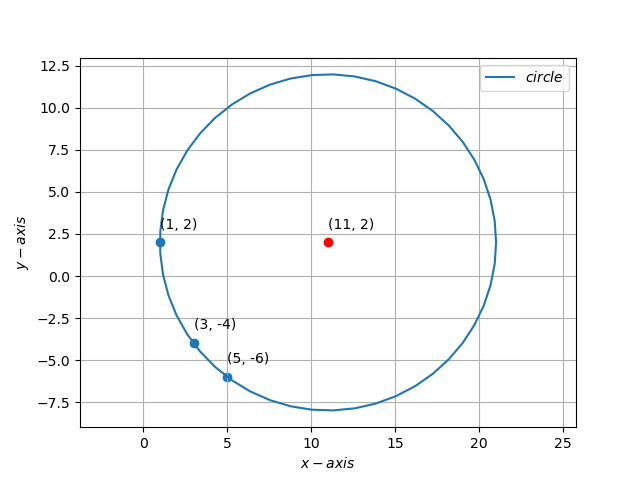
\includegraphics[width=\columnwidth]{solutions/17/16/Latex/Figure_1.png}
    \caption{Circle centered at $(11, 2)$ with radius $10$.}
    \label{eq:solutions/17/16/fig:1}
\end{figure}

